\FloatBarrier

\begin{figure}[h!]
	\centering
	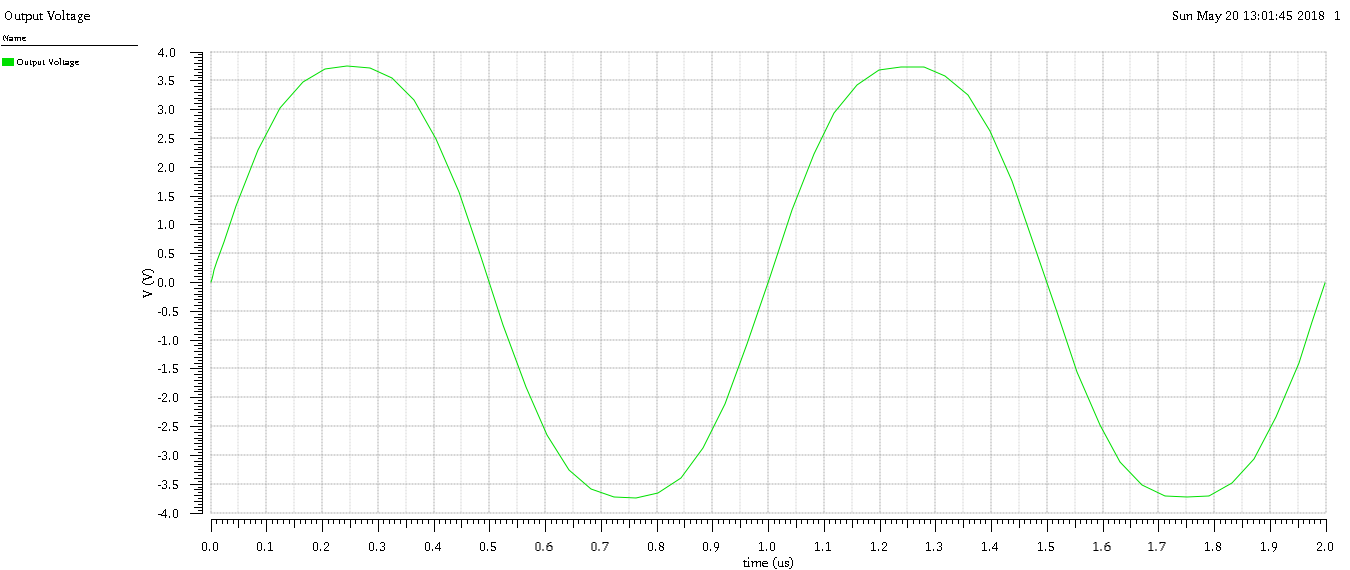
\includegraphics[scale=0.40]{./images/sim4_max_sin.PNG}
	\caption{Differential-Mode Output Waveform when $117.5$\si{\milli\volt} Differential-Mode Input Signal is Applied}
	\label{fig:sim4_max_sin}
\end{figure}

\FloatBarrier

The maximum amplitude of the applied signal is about $117.5$\si{\milli\volt}.
The corresponding maximum output amplitude is about $3.7$\si{\volt}.
The true value is likely even less because before the transistors enter triode or cutoff mode, distortions at the edge of the saturation region occur.
Past this point the amplifier begins to distort the output waveform and cause it to clamp.

\FloatBarrier

\begin{figure}[h!]
	\centering
	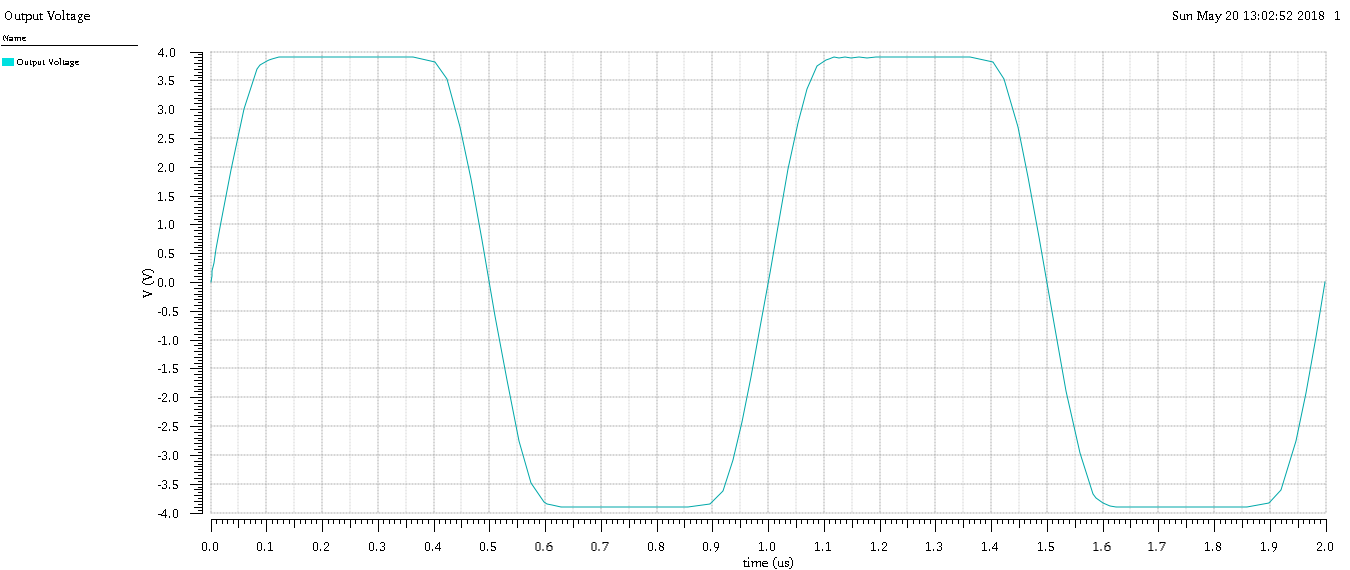
\includegraphics[scale=0.40]{./images/sim4_past_max.PNG}
	\caption{Significant Clamping of the Ouput Signal at $225$\si{\milli\volt}}
	\label{fig:sim4_past_max}
\end{figure}

\FloatBarrier
